\section{Minimum Cost Arborescences}\label{sec:3}

\subsection{Arborescences and a Characterization}\label{subsec:3.1}
Let $G = (V, E)$ be a directed graph and let $r$ be a distinguished 
node, which is commonly called a root. An {\bf arborescence} with respect to 
$r$ (or rooted at $r$) is a directed subgraph $T = (V, F)$ with $F \subseteq E$ 
such that 
\begin{enumerate}[(i)]
    \item undirected $T$ (that is, $T$ obtained from disregarding all directions) is a spanning tree; and 
    \item for every $v \in V$ with $v \neq r$, there is a directed path 
    in $T$ from $r$ to $v$. 
\end{enumerate}
For example, consider the following graph $G = (V, E)$. 
\begin{center}
    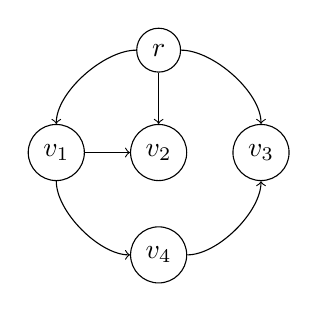
\begin{tikzpicture}[node distance={30mm}, main/.style = {draw, circle}] 
        \node[main] (r) at (0, 1.3) {$r$}; 
        \node[main] (1) at (-1.3, 0) {$v_1$};
        \node[main] (2) at (0, 0) {$v_2$};
        \node[main] (3) at (1.3, 0) {$v_3$};
        \node[main] (4) at (0, -1.3) {$v_4$};

        \draw[->] (r) to [out=180, in=90, looseness=0.75] (1);
        \draw[->] (r) -- (2);
        \draw[->] (r) to [out=0, in=90, looseness=0.75] (3);
        \draw[->] (1) -- (2);
        \draw[->] (1) to [out=270, in=180, looseness=0.75] (4);
        \draw[->] (4) to [out=0, in=270, looseness=0.75] (3);
    \end{tikzpicture} 
\end{center}
\vspace{-0.25cm}
Then the following two subgraphs are arborescences rooted at $r$.
\begin{center}
    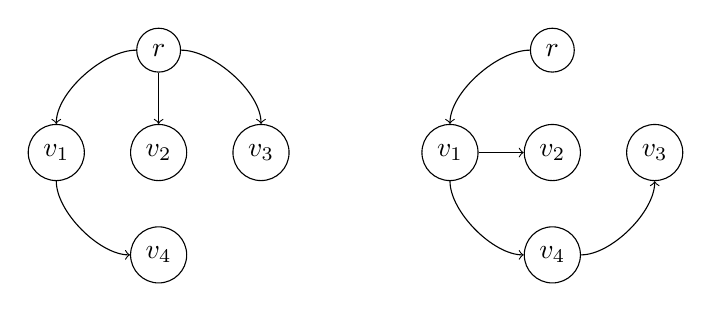
\begin{tikzpicture}[node distance={30mm}, main/.style = {draw, circle}] 
        \node[main] (r) at (0, 1.3) {$r$}; 
        \node[main] (1) at (-1.3, 0) {$v_1$};
        \node[main] (2) at (0, 0) {$v_2$};
        \node[main] (3) at (1.3, 0) {$v_3$};
        \node[main] (4) at (0, -1.3) {$v_4$};

        \node[main] (r') at (5, 1.3) {$r$}; 
        \node[main] (1') at (3.7, 0) {$v_1$};
        \node[main] (2') at (5, 0) {$v_2$};
        \node[main] (3') at (6.3, 0) {$v_3$};
        \node[main] (4') at (5, -1.3) {$v_4$};

        \draw[->] (r) to [out=180, in=90, looseness=0.75] (1);
        \draw[->] (r) -- (2);
        \draw[->] (r) to [out=0, in=90, looseness=0.75] (3);
        % \draw[->] (1) -- (2);
        \draw[->] (1) to [out=270, in=180, looseness=0.75] (4);
        % \draw[->] (4) to [out=0, in=270, looseness=0.75] (3);

        \draw[->] (r') to [out=180, in=90, looseness=0.75] (1');
        % \draw[->] (r') -- (2');
        % \draw[->] (r') to [out=0, in=90, looseness=0.75] (3');
        \draw[->] (1') -- (2');
        \draw[->] (1') to [out=270, in=180, looseness=0.75] (4');
        \draw[->] (4') to [out=0, in=270, looseness=0.75] (3');
    \end{tikzpicture} 
\end{center}
\vspace{-0.25cm}
On the other hand, the following two subgraphs are not arborescences
rooted at $r$: the first one is not a tree, and the second has no directed 
path from $r$ to $v_4$.
\begin{center}
    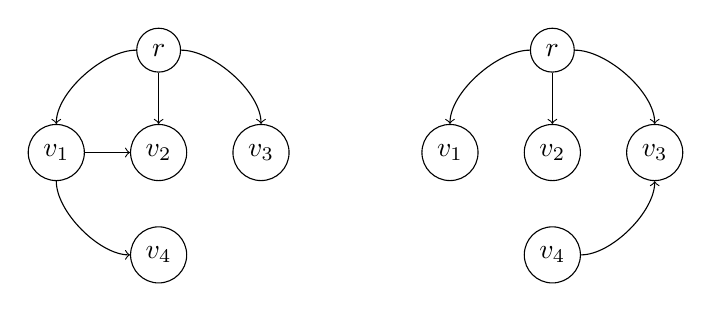
\begin{tikzpicture}[node distance={30mm}, main/.style = {draw, circle}] 
        \node[main] (r) at (0, 1.3) {$r$}; 
        \node[main] (1) at (-1.3, 0) {$v_1$};
        \node[main] (2) at (0, 0) {$v_2$};
        \node[main] (3) at (1.3, 0) {$v_3$};
        \node[main] (4) at (0, -1.3) {$v_4$};

        \node[main] (r') at (5, 1.3) {$r$}; 
        \node[main] (1') at (3.7, 0) {$v_1$};
        \node[main] (2') at (5, 0) {$v_2$};
        \node[main] (3') at (6.3, 0) {$v_3$};
        \node[main] (4') at (5, -1.3) {$v_4$};

        \draw[->] (r) to [out=180, in=90, looseness=0.75] (1);
        \draw[->] (r) -- (2);
        \draw[->] (r) to [out=0, in=90, looseness=0.75] (3);
        \draw[->] (1) -- (2);
        \draw[->] (1) to [out=270, in=180, looseness=0.75] (4);
        % \draw[->] (4) to [out=0, in=270, looseness=0.75] (3);

        \draw[->] (r') to [out=180, in=90, looseness=0.75] (1');
        \draw[->] (r') -- (2');
        \draw[->] (r') to [out=0, in=90, looseness=0.75] (3');
        % \draw[->] (1') -- (2');
        % \draw[->] (1') to [out=270, in=180, looseness=0.75] (4');
        \draw[->] (4') to [out=0, in=270, looseness=0.75] (3');
    \end{tikzpicture} 
\end{center}
\vspace{-0.25cm}
The following theorem gives us a useful characterization of arborescences.

\begin{theo}[Characterization of Arborescences]{theo:3.1}
    Let $G = (V, E)$ be a connected graph and let $T = (V, F)$ be a subgraph. 
    Then $T$ is an arborescence rooted at $r$ if and only if both 
    of the following conditions hold:
    \begin{enumerate}[(1)]
        \item every $v \in V$ with $v \neq r$ has exactly one incoming edge in $T$; and 
        \item $T$ has no directed cycles. 
    \end{enumerate}
\end{theo}
\begin{pf}[Theorem~\ref{theo:3.1}]
    $(\Rightarrow)$ First, we check that condition (1) holds. Consider a vertex 
    $v \in V$ with $v \neq r$. Since undirected $T$ is a spanning tree, 
    there is a unique (simple) path from $r$ to $v$ in undirected $T$. 
    The last edge on this path is incoming for $v$. Hence, all other edges 
    incident to $v$ in undirected $T$ should be outgoing edges for $v$ 
    (because the neighbours of $v$ also have unique simple paths from $v$ 
    to them in undirected $T$). This proves (1). To see that condition (2) 
    holds, note that undirected $T$ is acyclic as it is a spanning tree, 
    so it could not possibly have any directed cycles either. 

    $(\Leftarrow)$ Suppose that $V = (T, F)$ satisfies conditions (1) and (2). 
    First, we show that for all $v \in V$ with $v \neq r$, there exists 
    a directed path from $r$ to $v$ in $T$, which is condition (ii) of the 
    definition of an arborescence. Let $(v_1, v)$ be the unique edge 
    incoming to $v$ by condition (1), let $(v_2, v_1)$ be the unique edge 
    incoming to $v_1$, and so on. By contradiction, suppose that we 
    cannot reach $r$ by backtracking in this way. Then at some point, 
    we must visit the same node at least twice because $G$ is a finite graph. 
    But this creates a directed cycle, contradicting condition (2). Thus, 
    there is a directed path from $r$ to $v$ in $T$. 

    Now, we verify condition (i) that undirected $T$ is a spanning tree. 
    Note that we can get from $r$ to any other vertex $v$, so 
    undirected $T$ is connected. Moreover, $r$ has no incoming edges 
    because if $(v, r)$ is an incoming edge, then the directed path from 
    $r$ to $v$ followed by $(v, r)$ forms a directed cycle, contradicting 
    condition (2). Since every edge is incoming for exactly one of its 
    endpoints, the total number of edges in $T$ is 
    \[ \sum_{u=r} 0 + \sum_{\substack{u\in V \\ u\neq r}} 1 = |V| - 1. \] 
    By the fundamental theorem of trees (Theorem~\ref{theo:2.1}), 
    it follows that undirected $T$ is a spanning tree. \qed 
\end{pf}

\subsection{Minimum Cost Arborescences}\label{subsec:3.2}
Given a directed graph $G = (V, E)$, a distinguished node $r$, and edge 
costs $c_e \geq 0$ for each $e \in E$, our goal is to find an arborescence
rooted at $r$ so that the total edge cost is minimized. 

Let's try to transfer our knowledge from the minimum spanning tree problem. 
Do the analogues of the cycle and cut properties hold for arborescences?
It turns out we can find a counterexample to both in the same graph. 
Consider the following graph $G = (V, E)$ with associated edge costs. 
\begin{center}
    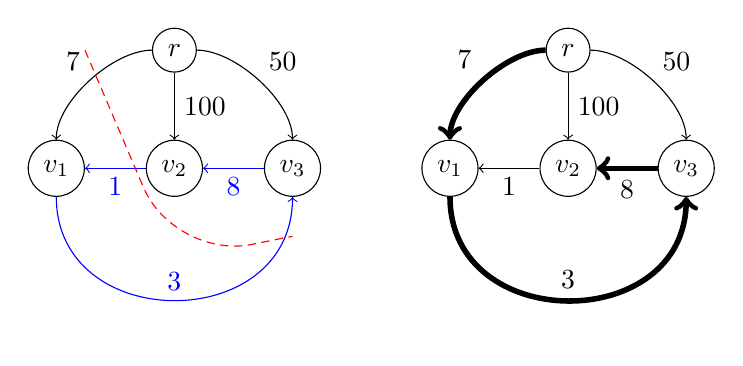
\begin{tikzpicture}[
        node distance={30mm}, 
        main/.style = {draw, circle},
        xs/.style = {xshift=#1 mm},
        ys/.style = {yshift=#1 mm}
    ] 
        \node[main] (r) at (0, 1.5) {$r$}; 
        \node[main] (1) at (-1.5, 0) {$v_1$};
        \node[main] (2) at (0, 0) {$v_2$};
        \node[main] (3) at (1.5, 0) {$v_3$};

        \node[main] (r') at (5, 1.5) {$r$}; 
        \node[main] (1') at (3.5, 0) {$v_1$};
        \node[main] (2') at (5, 0) {$v_2$};
        \node[main] (3') at (6.5, 0) {$v_3$};

        \draw[->] (r) to [out=180, in=90, looseness=0.75] node[midway, above left] {7} (1);
        \draw[->] (r) -- node[midway, right] {100} (2);
        \draw[->] (r) to [out=0, in=90, looseness=0.75] node[midway, above right] {50} (3);
        \draw[->, color=blue] (2) -- node[midway, below] {1} (1);
        \draw[->, color=blue] (3) -- node[midway, below] {8} (2);
        \draw[->, color=blue] (1) to [out=270, in=270, looseness=1.5] node[midway, above] {3} (3);

        \draw[rounded corners=10mm, red, densely dashed] 
            ([xs=-8.5] r.west) -- ([ys=-8] 2.south) -- ([ys=-5] 3.south);

        \draw[->, line width=2pt] (r') to [out=180, in=90, looseness=0.75] node[midway, above left] {7} (1');
        \draw[->] (r') -- node[midway, right] {100} (2');
        \draw[->] (r') to [out=0, in=90, looseness=0.75] node[midway, above right] {50} (3');
        \draw[->] (2') -- node[midway, below] {1} (1');
        \draw[->, line width=2pt] (3') -- node[midway, below] {8} (2');
        \draw[->, line width=2pt] (1') to [out=270, in=270, looseness=1.5] node[midway, above] {3} (3');
    \end{tikzpicture} 
\end{center}
\vspace{-0.25cm}
The minimum cost arborescence is given to the right with cost 
$7 + 3 + 8 = 18$. Consider the cut (in red) and cycle (in blue) above. 
Then the cut property fails to hold because the edge $(v_2, v_1)$ of cost $1$ was 
not picked in a minimum cost arborescence, and the cycle property fails 
to hold because the edge $(v_3, v_2)$ of maximum cost $8$ in the cycle 
was picked in a minimum cost arborescence. 

Can we instead consider the union of minimum cost incoming edges 
(vertex by vertex), excluding the root $r$? For the above example, 
if we start with $v_1$, we'd pick $(v_2, v_1)$ as it is the minimum cost 
edge incoming to $v_1$. Then $(v_1, v_3)$ is the minimum cost edge 
incoming to $v_3$ and $(v_3, v_2)$ is the minimum cost edge incoming to 
$v_2$. This yields the same directed cycle highlighted in blue above!

So this strategy does not immediately work. But if the strategy 
did happen to give us an arborescence, then we are already done! 
All we need to do is tweak it slightly. The idea is to compute 
\[ y_v = \min_{(u,v)\in E} c_{(u, v)} \] 
for all vertices $v \in V$ with $v \neq r$. In particular, any edge using this 
vertex needs to pay this cost anyways. Then for all $(u, v) \in E$, we can 
define new edge costs 
\[ c'_{(u, v)} = c_{(u, v)} - y_v. \] 
We give the edge costs $c'_e$ (in blue) and the values $y_v$ (in purple) for the above example.
Notice that some of the edges turn out to be free.
\begin{center}
    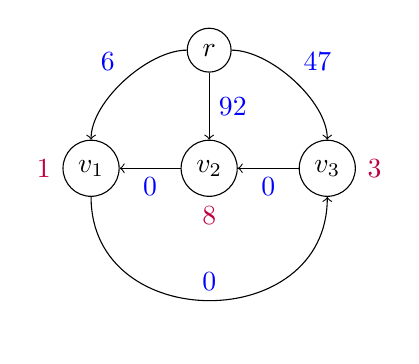
\begin{tikzpicture}[
        node distance={30mm}, 
        main/.style = {draw, circle},
    ] 
        \node[main] (r) at (0, 1.5) {$r$}; 
        \node[main] (1) at (-1.5, 0) {$v_1$};
        \node[color=purple] (1cost) at (-2.1, 0) {$1$};
        \node[main] (2) at (0, 0) {$v_2$};
        \node[color=purple] (2cost) at (0, -0.6) {$8$};
        \node[main] (3) at (1.5, 0) {$v_3$};
        \node[color=purple] (3cost) at (2.1, 0) {$3$};

        \draw[->] (r) to [out=180, in=90, looseness=0.75] node[midway, above left, text=blue] {6} (1);
        \draw[->] (r) -- node[midway, right, text=blue] {92} (2);
        \draw[->] (r) to [out=0, in=90, looseness=0.75] node[midway, above right, text=blue] {47} (3);
        \draw[->] (2) -- node[midway, below, text=blue] {0} (1);
        \draw[->] (3) -- node[midway, below, text=blue] {0} (2);
        \draw[->] (1) to [out=270, in=270, looseness=1.5] node[midway, above, text=blue] {0} (3);
    \end{tikzpicture} 
\end{center}
\vspace{-0.25cm}
Let's prove a useful result regarding these reduced edge costs. Its corollary 
will help us reason about the correctness of a minimum cost arborescence 
algorithm. 

\begin{lemma}{lemma:3.2}
    For every arborescence $T$ rooted at $r$, we have 
    \[ c(T) = c'(T) + \sum_{\substack{v\in V \\ v\neq r}} y_v. \] 
\end{lemma}\vspace{-0.15cm}
\begin{pf}[Lemma~\ref{lemma:3.2}]
    Splitting the sum to correspond to the individual vertices, we have 
    \[ c(T) = \sum_{e\in T} c_e = \sum_{(u, v) \in T} c_{(u,v)} 
    = \sum_{(u, r) \in T} c_{(u,r)} + \sum_{\substack{v\in V\\ v\neq r}} 
    \sum_{(u, v) \in T} c_{(u, v)}. \] 
    There are no edges directed to the root $r$ in an arborescence, so 
    the first sum is $0$. For the double summation, note that in an 
    arborescence, there is exactly one edge directed to each $v \in V$ 
    with $v \neq r$ by Theorem~\ref{theo:3.1}, so we only need to recompensate 
    $y_v$ once. This gives us 
    \begin{align*}
        c(T) &= \sum_{\substack{v\in V\\ v \neq r}} \left( \sum_{(u, v) \in T} (c_{(u, v)} - y_v) + y_v \right) \\
        &= \sum_{\substack{v\in V\\ v \neq r}} \sum_{(u, v) \in T} c'_{(u,v)} + \sum_{\substack{v\in V\\ v \neq r}} y_v 
        = c'(T) + \sum_{\substack{v\in V\\ v \neq r}} y_v,
    \end{align*}
    which is the desired result. \qed
\end{pf}

Since the sum of the vertex costs does not depend on the arborescence 
$T$, we obtain the following corollary. 

\begin{cor}{cor:3.3}
    An arborescence $T$ rooted at $r$ is of minimum cost with respect to 
    edge costs $c_e$ if and only if it is of minimum cost with respect 
    to the reduced edge costs $c'_e$. 
\end{cor}

\subsection{Edmonds' Algorithm}
From the ideas in the previous section, let's build
some intuition for Edmonds' algorithm before we state it. For each $v \neq r$, 
let $f_v = \argmin_{(u, v) \in E} c_{(u, v)}$ be an edge of minimum cost 
entering $v$. Let $F^* = \{f_v : v \neq r\}$ be the set of all of these 
minimum cost edges. Observe that by construction, all edges in $F^*$ have 
reduced edge costs $c'_e = 0$ since they attain the minimum cost 
and we are subtracting that minimum cost afterwards.

If $F^*$ does not contain a cycle, then it is a minimum cost arborescence 
rooted at $r$ by our characterization from Theorem~\ref{theo:3.1} and 
we are done. Otherwise, let $C$ be a cycle in $F^*$. Noting that all 
of the edges in $F^*$ are free with respect to the reduced edge costs, we can 
use as many of these edges as we want. So we can form a new graph 
$G' = (V', E')$ by contracting all the edges in $C$ into a supernode, and 
then recursively solve the problem for $G'$. After solving the problem 
for $G'$, we can extend it to an arborescence for $G$ by adding edges 
from the cycle $C$.

\begin{mdframed}[
    linewidth=1pt,
    linecolor=black,
    bottomline=false,topline=false,rightline=false,
    innerrightmargin=0pt,innertopmargin=0pt,innerbottommargin=0pt,
    innerleftmargin=1em,% Distance between vertical rule & proof content
    skipabove=0.75\baselineskip
]
{\bf Input.} A directed graph $G = (V, E)$, edge costs $c_e \geq 0$ for 
all $e \in E$, and a root node $r$. 

{\bf Output.} A minimum cost arborescence of $G$. 
\begin{enumerate}[leftmargin=1.75cm, label={Step \arabic*.}]
    \item {\bf (Initialization.)} 
    \begin{enumerate}[label={Step 1.\arabic*.}]
        \item {\bf (Find the minimum cost entering each vertex.)} 
        For each $v \in V$ with $v \neq r$, set 
        \begin{align*}
            y_v &\gets \min_{(u, v) \in E} c_{(u, v)}, \\ 
            f_v &\gets \argmin_{(u, v) \in E} c_{(u, v)}. 
        \end{align*}
        \item {\bf (Compute reduced edge costs.)} For each $(u, v) \in E$ 
        where $v \neq r$, set 
        \[ c'_{(u, v)} \gets c_{(u, v)} - y_v. \] 
        \item {\bf (Group edges of minimum cost.)} Set 
        \[ F^* \gets \bigcup_{\substack{v\in V\\ v\neq r}} f_v. \] 
        An equivalent way to see this is that for each $v \neq r$, we are picking 
        one edge $(u, v) \in E$ satisfying $c'_{(u,v)} = 0$.  
    \end{enumerate}

    \item {\bf (Recursive part of the algorithm.)}
    \begin{enumerate}[label={Step 2.\arabic*.}]
        \item {\bf (Base case.)} If $F^*$ is an arborescence rooted at $r$, 
        then stop and output $F^*$.
        \item {\bf (Recursive call.)} Let $C$ be a directed cycle in $F^*$
        (which exists by Theorem~\ref{theo:3.1}). 
        
        Contract $C$ to a supernode to obtain a graph $G' = (V', E')$, keeping 
        the reduced costs $c'_e$. 

        Recursively call Edmonds' algorithm to find a minimum cost arborescence 
        $F'$ for $G'$. Extend $F'$ to an arborescence for $G$ by adding 
        all but one edge in $C$. Then stop and return this arborescence.
    \end{enumerate}
\end{enumerate}
\end{mdframed}\vspace{-0.15cm}
Before we prove correctness, we'll first give a simple example of Edmonds' 
algorithm in action. 

Consider the following graph $G = (V, E)$ with associated edge costs $c_e$. \vspace{-0.15cm}
\begin{center}
    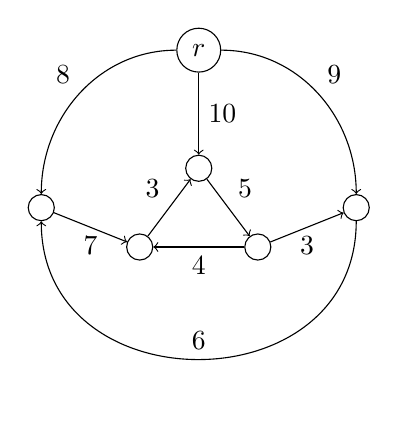
\begin{tikzpicture}[node distance={30mm}, main/.style = {draw, circle}] 
        \node[main] (r) at (0, 1.5) {$r$}; 
        \node[main] (1) at (-2, -0.5) {};
        \node[main] (2) at (0, 0) {};
        \node[main] (3) at (2, -0.5) {};
        \node[main] (4) at (-0.75, -1) {};
        \node[main] (5) at (0.75, -1) {};

        \draw[->] (r) to [out=180, in=90, looseness=1] node[midway, above left] {8} (1);
        \draw[->] (r) -- (2) node[midway, right] {10};
        \draw[->] (r) to [out=0, in=90, looseness=1] node[midway, above right] {9} (3);
        \draw[->] (1) -- node[midway, below] {7} (4);
        \draw[->] (4) -- node[midway, above left] {3} (2);
        \draw[->] (2) -- node[midway, above right] {5} (5);
        \draw[->] (5) -- node[midway, below] {3} (3);
        \draw[->] (5) -- node[midway, below] {4} (4);
        \draw[->] (3) to [out=270, in=270, looseness=1.5] node[midway, above] {6} (1);
    \end{tikzpicture} 
\end{center}
\vspace{-0.85cm}
In Step 1, we compute the minimum cost $y_v$ of entering each vertex $v \neq r$ 
and keep track of a set of edges $F^* = \{f_v : v\neq r\}$ that attain these minimums. 
We then set reduced edge costs $c'_e$. We'll label the edges in $F^*$ in bold, 
the values $y_v$ in purple, and the reduced edge costs $c'_e$ in blue. \vspace{-0.15cm}
\begin{center}
    \begin{tikzpicture}[node distance={30mm}, main/.style = {draw, circle}] 
        \node[main] (r) at (0, 1.5) {$r$}; 
        \node[main] (1) at (-2, -0.5) {};
        \node[color=purple] (1cost) at (-2.4, -0.5) {$6$};
        \node[main] (2) at (0, 0) {};
        \node[color=purple] (2cost) at (-0.3, 0.3) {$3$};
        \node[main] (3) at (2, -0.5) {};
        \node[color=purple] (3cost) at (2.4, -0.5) {$3$};
        \node[main] (4) at (-0.75, -1) {};
        \node[color=purple] (4cost) at (-0.75, -1.4) {$4$};
        \node[main] (5) at (0.75, -1) {};
        \node[color=purple] (5cost) at (0.75, -1.4) {$5$};
        \node[draw, dashed, inner sep=0pt, circle, yscale=0.95, fit={(2) (4) (5)}] {};

        \draw[->] (r) to [out=180, in=90, looseness=1] node[midway, above left, text=blue] {2} (1);
        \draw[->] (r) -- (2) node[midway, right, text=blue] {7};
        \draw[->] (r) to [out=0, in=90, looseness=1] node[midway, above right, text=blue] {6} (3);
        \draw[->] (1) -- node[midway, below, text=blue] {3} (4);
        \draw[->, line width=2pt] (4) -- node[midway, above left, text=blue] {0} (2);
        \draw[->, line width=2pt] (2) -- node[midway, above right, text=blue] {0} (5);
        \draw[->, line width=2pt] (5) -- node[midway, below, text=blue] {0} (3);
        \draw[->, line width=2pt] (5) -- node[midway, below, text=blue] {0} (4);
        \draw[->, line width=2pt] (3) to [out=270, in=270, looseness=1.5] node[midway, above, text=blue] {0} (1);
    \end{tikzpicture} 
\end{center}
\vspace{-0.85cm}
We have a directed cycle $C$ in $F^*$ indicated by the 
dotted circle above, so we must proceed to Step 2.2. This step tells us 
to contract $C$ to a supernode to obtain a graph $G' = (V', E')$
with the reduced edge costs $c'_e$. \vspace{-0.15cm}
\begin{center}
    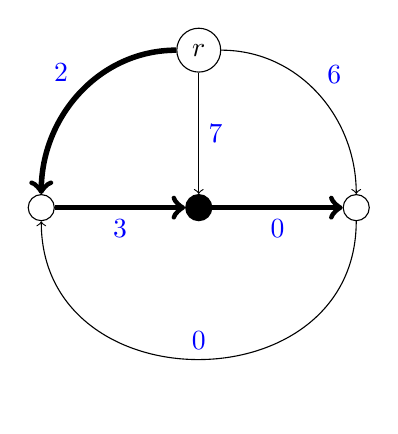
\begin{tikzpicture}[node distance={30mm}, main/.style = {draw, circle}] 
        \node[main] (r) at (0, 1.5) {$r$}; 
        \node[main] (1) at (-2, -0.5) {};
        \node[main] (3) at (2, -0.5) {};
        \node[main, fill=black] (6) at (0, -0.5) {};

        \draw[->, line width=2pt] (r) to [out=180, in=90, looseness=1] node[midway, above left, text=blue] {2} (1);
        \draw[->] (r) -- node[midway, right, text=blue] {7} (6);
        \draw[->] (r) to [out=0, in=90, looseness=1] node[midway, above right, text=blue] {6} (3);
        \draw[->, line width=2pt] (1) -- node[midway, below, text=blue] {3} (6);
        \draw[->, line width=2pt] (6) -- node[midway, below, text=blue] {0} (3);
        \draw[->] (3) to [out=270, in=270, looseness=1.5] node[midway, above, text=blue] {0} (1);
    \end{tikzpicture} 
\end{center}
\vspace{-0.85cm}
Here, we can find by inspection a minimum cost arborescence $F'$ for $G'$ of cost $5$,
highlighted in bold. Now we can extend $F'$ to an arborescence for $G$ 
by adding all but one edge in $C$. \vspace{-0.15cm}
\begin{center}
    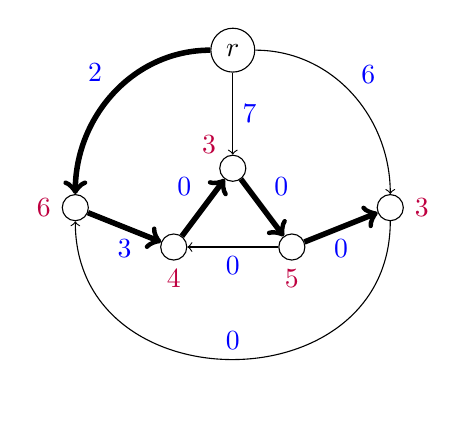
\begin{tikzpicture}[node distance={30mm}, main/.style = {draw, circle}] 
        \node[main] (r) at (0, 1.5) {$r$}; 
        \node[main] (1) at (-2, -0.5) {};
        \node[color=purple] (1cost) at (-2.4, -0.5) {$6$};
        \node[main] (2) at (0, 0) {};
        \node[color=purple] (2cost) at (-0.3, 0.3) {$3$};
        \node[main] (3) at (2, -0.5) {};
        \node[color=purple] (3cost) at (2.4, -0.5) {$3$};
        \node[main] (4) at (-0.75, -1) {};
        \node[color=purple] (4cost) at (-0.75, -1.4) {$4$};
        \node[main] (5) at (0.75, -1) {};
        \node[color=purple] (5cost) at (0.75, -1.4) {$5$};

        \draw[->, line width=2pt] (r) to [out=180, in=90, looseness=1] node[midway, above left, text=blue] {2} (1);
        \draw[->] (r) -- (2) node[midway, right, text=blue] {7};
        \draw[->] (r) to [out=0, in=90, looseness=1] node[midway, above right, text=blue] {6} (3);
        \draw[->, line width=2pt] (1) -- node[midway, below, text=blue] {3} (4);
        \draw[->, line width=2pt] (4) -- node[midway, above left, text=blue] {0} (2);
        \draw[->, line width=2pt] (2) -- node[midway, above right, text=blue] {0} (5);
        \draw[->, line width=2pt] (5) -- node[midway, below, text=blue] {0} (3);
        \draw[->] (5) -- node[midway, below, text=blue] {0} (4);
        \draw[->] (3) to [out=270, in=270, looseness=1.5] node[midway, above, text=blue] {0} (1);
    \end{tikzpicture} 
\end{center}
\vspace{-0.35cm}
Corollary~\ref{cor:3.3} tells us that working with the reduced edge costs 
$c'_e$ still gives us a minimum cost arborescence for the original edge 
costs $c_e$, so Step 1 is valid. 

Moreover, note that the reduced edge costs $c'_e$ are all nonnegative 
and $c'_e = 0$ for all $e \in F^*$, meaning that if $F^*$ happened to be 
an arborescence rooted at $r$ at Step 2.1, then it is an arborescence 
of cost $0$. In particular, every other arborescence also has nonnegative 
cost with respect to $c'_e$, so $F^*$ would be a minimum cost arborescence. 

Arguing the correctness of Step 2.2 is trickier. One concern is that 
contracting the cycle $C$ places extra constraints on the 
arborescence. A minimum cost arborescence in $G'$ must have exactly 
one edge entering the contracted supernode corresponding to $C$. 
However, a minimum cost arborescence for $G$ might have several edges 
entering $C$. To resolve this, we have the following lemma. 

\begin{lemma}{lemma:3.4}
    Let $C$ be a cycle consisting of edges $e$ with $c'_e = 0$, and 
    suppose that $r \notin C$. Then there is a minimum cost arborescence 
    rooted at $r$ that has exactly one edge incoming to $C$.
\end{lemma}\vspace{-0.15cm}
\begin{pf}[Lemma~\ref{lemma:3.4}]
    Let $T$ be a minimum cost arborescence in $G$. By definition, there is a 
    directed $r,v$-path to every vertex $v \neq r$ in $T$, so at least one 
    edge enters $C$. If exactly one edge enters $C$, then we are done by taking $T$. 

    Suppose now that there are at least two edges entering $C$. We will 
    construct another minimum cost arborescence $T'$ that has exactly 
    one edge entering $C$. Let $(u, v)$ be an edge in $T$ entering $C$ 
    that lies on a shortest path from $r$ to $C$. Note that this path from 
    $r$ to $C$ uses only one vertex in $C$. Delete all the edges that 
    enter a vertex in $C$ except for $(u, v)$ from $T$, and add in 
    edges of $C$ except for the one that enters $v$. 

    We claim that $T'$ is a minimum cost arborescence. Note that we are 
    only adding edges with cost $c'_e = 0$, so $c'(T) \geq c'(T')$. 
    By construction, $T'$ has no directed cycles because $T$ had no cycle 
    before and had no cycles within $C$, and now only $(u, v)$ enters $C$. 
    Moreover, there is exactly one edge entering each vertex $v \neq r$ 
    because for every vertex on $C$, we either did nothing or added 
    and removed an edge entering $v$. By Theorem~\ref{theo:3.1}, $T'$ is 
    also a minimum cost arborescence with exactly one edge incoming to $C$. \qed
\end{pf}\vspace{-0.25cm}

Another concern: does an arborescence $F'$ rooted at $r$ in the graph 
$G'$ might not give us an arborescence $F$ rooted at $r$ in $G$? It turns 
out this is always the case; we leave the proof of the following lemma 
as an exercise. The idea is to consider the edges in the cycle $C$, which 
we know have reduced edge costs $c'_e = 0$. 

\begin{lemma}{lemma:3.5}
    Every arborescence $F'$ rooted at $r$ in the graph $G'$ leads to 
    an arborescence $F$ rooted at $r$ in $G$ such that $c'(F') = c'(F)$. 
\end{lemma}\vspace{-0.15cm}
